\documentclass[pfc]{imetex}
\usepackage[table]{xcolor}
\usepackage{graphicx}

%% Capa
\firstAuthor{Victor Villas Bôas Chaves}
\secondAuthor{Lucas Sousa Meireles}
\thirdAuthor{Claudio Cavalcante Bomfim Júnior}

\title{Serviço de Análise Comportamental baseado em Dinâmica de Digitação para Arquiteturas de Autenticação Multifator}
\date{Outubro 2017}

%% Folha de Rosto
\preamble{Projeto de Final de Curso apresentado ao Curso de Egenharia de Computação do Instituto Militar de Engenharia, como requisito parcial para a obtenção do título de Engenheiro de Computação.}
\advisor{Prof. Ronaldo Goldschmidt}

%% Resumo
\vernacularAbstract{
}
\vernacularKeywords{dinâmica da digitação, reconhecimento de usuário}
\vehicularAbstract{
}
\vehicularKeywords{keyboard dynamics, user authentication}

%% Referências
\references{pfc}

\begin{document}

\chapter{Introdução}

\section{Contexto e Motivação}
Autenticação é o processo de verificar positivamente a identidade de um usuário, dispositivo ou outra entidade em um sistema computacional, em geral como prerequisito de permissão de acesso a recursos. A autenticação de uma entidade alcança verificação positiva ao corretamente corresponder uma forma de identificação (como uma chave secreta) previamente definida. \cite{OGorman2003}

É conveniente discernir a diferensa entre autenticação de dispositivos (máquinas) e usuários (pessoas), sendo o último sistema onde concentram-se diversas dificuldades em função da usabilidade e interface para o usuário. \cite{OGorman2003} O uso de senhas que humanos possam lembrar é por si só um fator de risco, havendo portanto a necessidade de introduzir mecanismos secundários de autenticação que não introduzam queda de usabulidade significativa \cite{Morris1979}.


Dentre as alternativas de autenticação multifator, o uso de características biométricas se destaca por sua natureza individual e difícil falsificação. Utilizados principalmente em sistemas de autorização e autenticação em ambientes físicos, um sistema biométrico se baseia em um sensor consistente de assinatura biométrica \cite{EdDawson2003}.

As características biométricas frequentemente mencionadas são as fisiológicos, mas seu emprego traz diversos fatores complicantes como a necessidade de amostragem prévia e diminuição da usabilidade do sistema. Uma alternativa é o uso de características biométricas de comportamento, como padrões comportamentais expressos naturalmente pelo usuário \cite{Moskovitch2009}.

As vantagens do uso de características comportamentais incluem a possibilidade de amostragem silenciosa, maior variabilidade do grau de confiança e a transparência do mecanismo para o usuário, o campo da segurança da informação mantém-se sem muitos meios de autenticação neste sentido. Em particular, sistemas providos pela \textit{Web} em geral possuem uma uniformidade de interface que permite a coleta de vários padrões comportamentais durante todo o uso do sistema \cite{Moskovitch2009}.	


\section{Objetivos}
Esse trabalho tem como principal objetivo a construção de um sistema de autenticação baseado em dinâmica de digitação do usuário, disponibilizado como serviço externo interagindo através de uma API, além de desenvolver uma biblioteca que facilite sua integração a outros componentes de serviços Web, e conta como objetivos secundários os eguintes tópicos:

\begin{itemize}
\item Analisar os tipos de informação que se podem extrair a partir dos padrões de digitação de um indivíduo;
\item Modelar a combinação das informaçoes extraídas utilizando algoritmos de aprendizado de máquina;
\item Sistematizar um mecanismo de coleta de amostras que permita o treinamento dos modelos escolhidos;
\item Definir uma arquitetura de sistema para implantação dos mecanismos de coleta e autenticação definidos;
\end{itemize}

\section{Contribuições Esperadas}
Espera-se desse projeto a produção de um mecanismo de autenticação com total transparencia ao usuário, como um serviço complementar de autenticação do mesmo, com a finalidade de impedir fraudes de acesso as aplicações do cliente, sem que o usuário esteja ciente da aplicação. Deste modo o agente malicioso não tomará conhecimento deste segundo método de autenticação e não estará apto a se adaptar ao padrão de digitação de quem este pretende invadir, o projeto visa assim suprir a necessidade de autenticação transparente da qual carece o mercado de segurança da informação, por meio de padrões compartamentais, os quais são mais difíceis de se simular.  

\section{Método}
O desenvolvimento do serviço de autenticação e da biblioteca será feito de forma paralela. Por um lado a biblioteca é responsável por coletar os dados de dinâmica de digitação no navegador de um usuário, enquanto o serviço receberá esses dados e fará a verificação de identidade.

Após a arquitetura do sistema estar definida, serão experimentados modelos de aprendizado de máquina em um serviço protótipo para prova de conceito. Durante esse experimento poderá ser feita coleta de dados e ao mesmo tempo avaliar a usabilidade da biblioteca.

\section{Viabilidade}
O desenvolvimento da biblioteca de interação com a API, por ser um  produto independente do desenvolvimento do sistema de autenticação, pode ser ajustado conforme a disponibilidade de tempo do projeto. Portanto, a viabilidade do projeto se dá principalmente como dependente da prototipagem e experimentação do sistema.

Como o IME possui diversas oportunidades de experimentação com seus alunos em ambiente EAD, o experimento é factível e pode ser feito nos moldes de trabalhos semelhantes anteriores. Em todo caso, há \textit{datasets} públicos de dinâmica de digitação que podem ser utilizados caso o desenvolvimento do sistema ultrapasse o cronograma esperado e inviabilize a coleta de dados local.

\section{Cronograma}
\begin{table}[htb]
\begin{tabular}{|l|c|c|c|c|c|c|c|c|c|}
\hline
& Fev & Mar & Abr & Mai & Jun & Jul & Ago & Set & Out \\
\hline
Revisão bibliográfica &
%\multicolumn{0}{c}{} &
\multicolumn{2}{c}{\cellcolor[gray]{0.5}} &
\multicolumn{6}{c}{} &
\\
\hline
Modelagem conceitual &
\multicolumn{1}{c}{} &
\multicolumn{3}{c}{\cellcolor[gray]{0.5}} &
\multicolumn{4}{c}{} &
\\
\hline
Prototipagem &
\multicolumn{2}{c}{} &
\multicolumn{3}{c}{\cellcolor[gray]{0.5}} &
\multicolumn{3}{c}{} &
\\
\hline
Coleta de dados &
\multicolumn{4}{c}{} &
\multicolumn{1}{c}{\cellcolor[gray]{0.5}} &
\multicolumn{3}{c}{} &
\\
\hline
Entrega de relatório parcial &
\multicolumn{3}{c}{} &
\multicolumn{1}{c}{\cellcolor[gray]{0.5}} &
\multicolumn{1}{c}{} &
\multicolumn{1}{c}{\cellcolor[gray]{0.5}} &
\multicolumn{2}{c}{} &
\\
\hline
Experimentação &
\multicolumn{5}{c}{} &
\multicolumn{2}{c}{\cellcolor[gray]{0.5}} &
\multicolumn{1}{c}{} &
\\
\hline
Entrega do relatório final &
\multicolumn{7}{c}{} &
\multicolumn{1}{c}{\cellcolor[gray]{0.5}} &
%\multicolumn{1}{c}{} &
\\
\hline
Apresentação &
\multicolumn{8}{c}{} &
\multicolumn{1}{c}{\cellcolor[gray]{0.5}}
%\multicolumn{7}{c}{} &
\\
\hline
\end{tabular}

\caption{Cronograma mensal de trabalho}
\end{table}

\begin{table}[htb]
\begin{tabular}{|l|c|}
\hline
Definição da arquitetura básica do produto & VE\\
\hline
Coletanea de trabalhos relacionados ao tema proposto & VC\\
\hline
Prototipagem do serviço de autenticação & VC\\
\hline
Escolha dos modelos de aprendizado de máquina & VC\\
\hline
Esquematização da API e modelagem do sistema & VC\\
\hline
Experimentação do serviço via API em um ambiente simulado & VF\\
\hline
Análise dos resultados e reltório da efetividade do sistema & VF\\
\hline
\end{tabular}

\caption{Tarefas entregáveis}
\end{table}


\section{Organização do Texto}
No capítulo \ref{fundamentaca} são introduzidos os conceitos necessários para a modelagem conceitual de um sistema de autenticação por dinâmica de digitação. Na seção \ref{relacionados} são discutidos trabalhos relacionados.

No capítulo \ref{solucao} é apresentado uma arquitetura de sistema de autenticação isolado, para fácil implantação do método apresentado. Na seção \ref{modelo} é definido o modelo de autenticação, especificando o fluxo de informações desde a coleta até a decisão de um grau de confiança de identidade, enquanto em \ref{prototipo} é demonstrada uma possível implementação da solução proposta, servindo como prova de conceito para o modelo.

No capítulo \ref{experimentos} são analisados os resultados do experimento proposto com o protótipo criado, analisando o sucesso da solução.

No capítulo \ref{conclusao} termina-se por sumarizar o conceito, a solução e os resultados obtidos pelo sistema apresentado.

\chapter{Fundamentação}
   O problema que o ramo de aprendizado por máquinas se propõe a resolver é a busca pela aproximação funcional matemática de um problema real em um conjunto matemático, onde $F:C \rightarrow R$ é a função alvo desconhecida, então para resolver o problema é suposto uma função $G:H \rightarrow R$, onde $G$ é a função estimada que pretende-se aproximar de $F$, $H \subset C$ é o conjunto das amostras que pretende-se expandir para o conjunto real expandido $C$, os valores de $H$ e $R$ são conhecidos; porém, para um problema não interpolável, não há um mapeamento conhecido de $F:C \rightarrow R$, seja por falta parâmetros de difícil análise, ou pelo caráter indeterminado do problema, em ambos os casos o tratamento é similar atravéz de estimação e tratamento de erros na abordagem.

\section{Problema de Classificação}

    O problema de traduzir um conjunto amostral $H$ em conjuntos distintos com uma abordagem não interpolável é conhecido como o problema classificação, para tal pode se usar, no domínio discreto, a seguinte abordagem. Seja $f: x->y$ a função alvo onde $x = [x_1,x_2,...,x_d]^t$ é o vetor das amostras de $H$, seja o somatório $\sum\limits_{i=1}^d \omega_i*x_i$, onde $\omega_i$ é o peso do seu respectivo elemento do vetor $x$, de tal forma que:

    \begin{equation}
        \sum\limits_{i=1}^d \omega_i*x_i>t; y = 1.
        \sum\limits_{i=1}^d \omega_i*x_i<t; y = 0.
    \end{equation}

    De tal forma os pesos tem suas características definidas por seus respectivos elementos de $x$ da seguinte forma:\newline
    $|\omega_i|$ é alto quando $x_i$ for importante.\newline
    $\omega > 0$ quando $x_i$ for benéfico.\newline
    $\omega < 0$ quando $x_i$ for maléfico.\newline
    Por fim teremos uma aproximação da função alvo no problema de classificação para $h(x) = sign((\sum\limits_{i=1}^d \omega_i*x_i)+\omega_0)$, onde $\omega_0 = t$.

    Neste caso o problema de classificação se restringirá a apenas dois conjuntos alvo em $R$, para uma generalização com múltiplos conjuntos usam-se estratégias de modo a recair no problema com dois conjuntos alvo.

\section{Erro de amostragem}

    Vale notar que o vetor $x$ apenas representa as amostras colhidas, assim embora ele represente o conjunto $C$ como uma aproximação de $C$ para $H$ existe uma divergência conhecida como erro dentro da amostra $E_in$ essa diferença é representada pela diferença entre $x$ e sua projeção em $C$, assim como a extrapolação da função nem sempre vai atender o comportamento esperado pela função estimada $G: H \rightarrow R$ assim a divergência entre o real e o esperado é o chamado fora da amostra $E_out$, o qual funciona como um meio de verificar o quão errada esta a estimação de $G: H \rightarrow R$.

    Em um problema de aprendizado a verificação de erros não é um problema trivial, uma vez que pela impossibilidade de se conferir ambos os erros, $E_{in}$ e $E_{out}$, de maneira direta, por não conhecermos a função alvo, usam-se ferramentas que possibilitam verificar tais erros e assim modificar de maneira eficiente o método de estimação da função, uma primeira ferramenta usada para verificação de erros é a desigualdade de Hoeffding Chernoff como meio de verificação sobre os erros dentro e fora da amostra, a desigualdade em questão pode ser expressa da seguinte forma:

    \begin{equation}
        \begin{split}
            & P[|\upsilon - \mu|>\epsilon] \leq 2*e^{-2*\epsilon^2*N}, \epsilon>0 \\
            & P[|\upsilon - \mu|\leq\epsilon] > 2*e^{-2*\epsilon^2*N}, \epsilon>0
    \end{split}
    \end{equation}
    \newline
    A fim de melhor adaptar os valores, leia-se $P[x]$ como probabilidade de $x$, e diminuir os erros escolhe-se o valor de $\epsilon$ de tal forma que $\upsilon + \epsilon \geq \mu \geq \upsilon - \epsilon$, nota-se que a fronteira denotada por $2*e^{-2*\epsilon^2*N}$ não depende de $\mu$, nem do tamanho do domínio.
    \newline
    Adaptando-se a desigualdade ao problema de classificação ela é reescrita de forma que $|E_{in}-E_{out}|=|\upsilon-\mu|$ assim tem-se:
    \begin{equation}
        \begin{split}
             & P[|E_{in}-E_{out}|>\epsilon] \leq 2*|H|*e^{-2*\epsilon^2*N} \\ & P[|E_{in}-E_{out}|\leq\epsilon] > 2*|H|*e^{-2*\epsilon^2*N}, \epsilon>0
        \end{split}
    \end{equation}

    Como o erro $E_in$ é uma medida que advem da diferença entre a projeção da função estimada pode há uma identidade para tal, na qual o $E_in$ é a média das distâncias entre o valor real e o estimado, os seja:
    \begin{equation}
        \begin{split}
            & E_{in} = \frac{\sum\limits_{i=0}^N L(g(x_i),f(x_i))}{N} \\
            & E_{in} = \frac{\sum\limits_{i=0}^N L(g(x_i),y_i)}{N}
        \end{split}
    \end{equation}
    Quando a função alvo é indeterminada, dessa forma como o $E_{in}$ é independente de $E_{out}$ além de ser identicamente distribuída a tal pode-se afirmar que o valor de $E_{out}$ converge para $E_{out} = E(E_{in}) = E(\frac{\sum\limits_{i=0}^N L(g(x_i),y_i)}{N})$, leia $E(x)$ como a esperança de $x$, logo o erro de classificação é representado como $P[g(x) \neq y] = E(L(g(x),y))$ de tal forma para minimizar de maneira mais eficiente se estipula parametros afim de diminuir o erro quadrático médio assim buscam-se os parâmetros, tais que $(x, y) \rightarrow inf E((y-g(x))^2)$, leia-se $inf$ como infimo.

    Afim de otimizar a estimação busca-se então um classificador ótimo ao problema tal que o $E_{out}$ seja mínimo sem para isso alterar a amostra, de tal forma $E_{out}^{*} = inf( E_{out}(h))$, $h \in H$ nesse caso o erro fora da amostra é minimizado quando ele se aproxima do erro para um classificador ótimo $inf(E_{out}-E_{out}^{*})$, seja $\overline{h} \in H$, tal que $\overline{h}$ é a amostra ideal, nesse caso $E_{out}-E_{out}^{*} = (E_{out} - E_{out}(\overline{h})) + (E_{out}(\overline{h}) - E_{out}^{*})$, onde $E_{out} - E_{out}(\overline{h})$ é o erro na estimação da amostra e $E_{out}(\overline{h}) - E_{out}^{*}$ o erro na aproximação da amostra, assim minimizar o erro de estimação implica em aumentar o erro de aproximação, bem como assim minimizar o erro de aproximação implica em aumentar o erro de estimação, no entanto o erro de estimação esta diretamente ligado ao $E_{in}$, portanto minimizar o $E_{in}$ e consequentemente o $E_{out}$ implicam em aumento do erro de aproximação, logo existe um risco associado quando se tenta adaptar a função estimada ao comportamento real, o que pode levar ao problema de overfitting, para impedi-lo avalia-se então o risco associado a relação entre os erros conforme aa seguinte forma:
    \begin{equation}
        E_{out} - E_{out}^{*} \leq E_{out} - E_{in} - E_{out}^{*} + E_{in}^{*} \leq Sup(|E_{out}-E_{in}|)
    \end{equation}

    Assim usando-se da desigualdade $(3)$ para isolar o valor de $\epsilon$, tem-se que o valor de $Sup(|E_{out}-E_{in}|)$ substituindo o valor $\epsilon$ na equação resultante chega-se a:
    \begin{equation}
        Sup(|E_{out}-E_{in}|) \leq \alpha \sqrt{\frac{log(|H|)}{N\delta}}
    \end{equation}   

    Dessa forma é possível limitar a variação máxima entre os dois erros afim de minimizar o risco associado ao overfitting, para usar essa relação de maneira formal no ambito do problema ainda é preciso analisar as caraterísticas do conjunto $H$, de onde são colhidas as amostras para teste e treino, para tal busca-se a divisão em subconjuntos de maneira que estes sejam disjuntos e $H$ é então separado como um conjunto, tal que $H(s) = \{ h(x_1), h(x_2), ..., h(x_N) \}$, com $s \in X^N$, assim o crescimento de $H$ será delimitado por $2^N$ e consequentemente o seu número de dicotomias ($m_h(H)$), que são as formas de separar $H$ em duas partes, será a forma de se avaliar o crescimento de $H$ afim de reduzir os riscos ao selecionar a abordagem e tratar os erros do problema de classificação.

    \section{Dimensão de Vapnik-Charvanenks ($D_{vc}$)}

    Ainda assim é necessária uma ferramenta que defina qual o maior subconjunto de $H$, o qual possa ser separado dicotomicamente em $H$, pois a análise anterior foi feita integralmente com base no supremo da diferença entre os erros em $H$ para tal foi criada a dimensão de Vapnik-Charvanenks, assim:
    \begin{equation}
        \begin{split}
            & d_{vc}(H) = max\{N:m_H\} \\
            & d_{vc}(H) = \infty, se (m_h(N)=2^N, \forall N)
        \end{split}
    \end{equation}

    a dimensão VC em sí é uma ferramente de difícil estimação, para facilitar a sua utilização em vista da minimização de risco  é utilizado o Lema de Sauer, tomando $d_{vc}=d$, implicando em:
    \begin{equation}
        m_h(N) \leq \sum_{i=0}^d {\left(\begin{split} & N \\ & i\end{split}\right)} = \phi_d(N) \leq \left( \frac{eN}{d} \right)^d
    \end{equation}
    Ainda assim o ajuste ainda estará sujeito a erros de generalização quando a tese escolhida $G: H \rightarrow C$, quando for colocado em prática, tal erro é exposto como erro de generalização denotado como $arg Min E_{in}(h) = arg_{h \in H} \frac{1}{N}\sum L(h(x),y) $, leia $Min$ como mínimo, a fim de minimizar esses erros bem como seus riscos tornam-se necessárias táticas de verificação e validação da tese.

    \section{Validação}

    A validação é uma técnica que visa tornar a tática escolhida em otimal, assim sendo a validação é principalmente um meio de garantir que a abordagem escolhida para o problema esteja tão próxima da realidade quanto for possível, neste caso o conjunto de amostras é tratado para aprimorar a aplicação da tática, o tratamento pode funcionar de maneiras de ferentes de uma tática para outra, por fim a tática de validação mais utilizada e precisa quanto a validar o modelo é a validação cruzada, a qual apesar da eficiência e precisão pode não ser utilizada em detrimento de outras táticas por ser muito custosa em termos computacionais.

    A validação cruzada se baseia em redistribuir a amostra de teste em diversas sub-amostras de treino para então escolher-se recursivamente tais conjuntos de amostras e usar o restante como amostra de treino esta abordagem visa estimar o valor do $E_{out}$ que não pode ser calculado sem treino ou verificação do modelo já em uso, então calculam-se os erros para assim se escolher como amostra de teste a amostra, a qual contenha os melhores índices de erro; porém, como visto previamente, forçar os valores de erro na amostra e fora dela para minimiza-los pode acarretar em problemas de overfitting e neste caso os erros calculados durante a validação iriam distuar drasticamente do seu valor real.

    Outra técnica de validação amplamente utilizada é a reamostragem, nesse caso o modelo escolhido, mesmo após processos de verificação, não atende as espectativas quando implementado e por isso necessita-se refazer o treinamento, assim sendo se colhem novas amostras para refazer o processo de treino, é importante que não se usem as amostras já colhidas, pois estas iriam moldar o novo modelo com certo juízo de valor, contribuindo fatalmente para o problema de overfitting.

    Outra forma de validar um modelo é pela verificação continua durante o treino, neste caso a cada iteração do treinamento calculam-se os erros  do modelo em relação ao esperado para assim melhorar o modelo com alterações pontuais, similar ao processo de entraga de um produto em que a cada versão busca-se melhora-lo e consertar os problemas descobertos, assim como a tática de validação cruzada esse método é muito custoso computacionalmente e por isso pode ser desestimulado em relação aos outros.
    
\label{fundamentaca}


\section{Trabalhos Relacionados}

\label{relacionados}


\chapter{Solução Proposta}
\label{solucao}


\begin{center}
    \noindent\makebox[\textwidth]{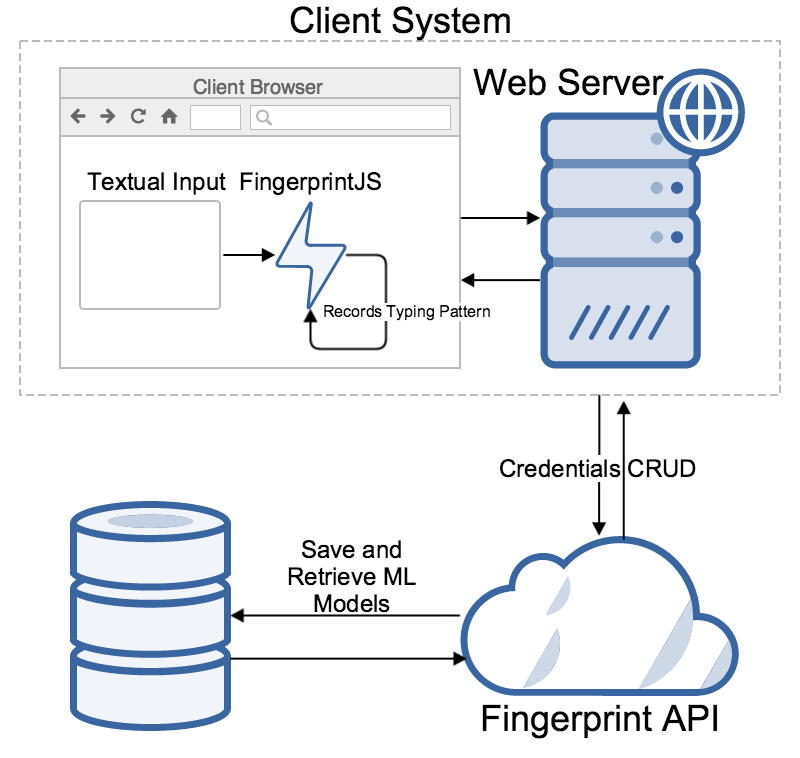
\includegraphics[width=8cm]{SystemDesign.png}}
\end{center}

\section{Modelo conceitual}
\label{modelo}


\section{Protótipo}
\label{prototipo}


\chapter{Experimentos e Resultados}
\label{experimentos}

\chapter{Conclusão}
\label{conclusao}


\end{document}
